\documentclass[12pt]{article}
\usepackage[utf8]{inputenc}
\usepackage{amsmath}
\usepackage{amsfonts}
\usepackage{amssymb}
\usepackage{empheq}
\usepackage{tikz}
\usepackage{enumitem}
\usepackage{eucal}
\usepackage{changepage}
\usetikzlibrary{automata, positioning, shapes}
\addtolength{\topmargin}{-0.75in}
\addtolength{\textheight}{1.75in}
\addtolength{\evensidemargin}{-0.5in}

\title{Topology Homework 06}
\author{Ethan Jensen, Luke Lemaitre, Kasandra Lassagne}
\date{March 11, 2020}

\begin{document}
  \maketitle
  \noindent
  \textbf{EXERCISE 3.1}
  Let \(X = \{(x,0)\in \mathbb{R}^2|\ x \in \mathbb{R}\}\), the x-axis in the plane. Describe the topology that \(X\) inherits as a subspace of \(\mathbb{R}^2\) with the standard topology.
  \newline \newline
  \(X\) inherits the standard topology on \(\mathbb{R}\).
  \newpage
  \noindent
  \textbf{EXERCISE 3.2}
  Let \(Y = [-1,1]\) has the standard topology. Which of the following sets are open in \(Y\) and which are open in \(\mathbb{R}\)?
  \begin{adjustwidth}{1cm}{0cm}
    \begin{flushleft}
      \(A = (-1,-1/2) \cup (1/2,1)\) \newline
      \(B = (-1,-1/2] \cup [1/2,1)\) \newline
      \(C = [-1,-1/2) \cup (1/2, 1]\) \newline
      \(D = [-1,-1/2] \cup [1/2,1]\) \newline
      \(E = \bigcup_{n=1}^\infty(\frac{1}{1+n}, \frac{1}{n})\)
    \end{flushleft}
  \end{adjustwidth}
  \(\ \)
  \newline
  \boxed{\textup{A, C, and E are open in Y}}
  \newline
  \boxed{\textup{A and E are open in } \mathbb{R}}
  \newpage
  \noindent
  \textbf{EXERCISE 3.3}
  \textbf{Prove Theorem 3.4:} Let X be a topological space, and let \(Y \subseteq X\) have the subspace topology. Then \(C \subseteq Y\) is closed in \(Y\) if and only if \(C = D \cap Y\) for some closed set \(D\) in \(X\).
  \newline \newline
  \textbf{Proof.}
  \newline
  \((\rightarrow)\)\ Assume C is closed in Y.
  \newline
  Let \(L_Y\) be the set of limit points of C in Y.
  \newline
  Let \(L_X\) be the set of limit points of C in X.
  \newline
  By Theorem 2.8, Cl\((C)\) in Y = \(C \cup L_Y\) and Cl\((C)\) in X = \(C \cup L_X\).
  \newline
  Since \(Y \subseteq X,\ L_Y = L_X \cap Y\).
  \newline \newline
  Let D be Cl\((C)\) in X. This makes D closed in X.
  \newline
  Notice that \(D \cap Y = (C \cup L_X)\cap Y = (C \cap Y) \cup (L_X \cap Y) = C \cup L_Y\)
  \newline
  This means \(D \cap Y =\) Cl\((C)\) in Y.
  \newline
  Since C is closed in Y, Cl\((C)\) = C.
  \newline
  \newline
  Thus, \(C = D \cap Y\) for some closed set \(D\) in \(X\).
  \newline \(\square\) \newline
  \((\leftarrow)\)\ Assume \(C = D \cap Y\) for some closed set \(D\) in \(X\).
  \newline
  Since D is closed in X, \(X - D\) is open in X.
  \newline
  By the definition of the subspace topology, \((X-D)\cap Y\) is open in Y.
  \newline
  So \(Y-D\) is open in Y, so its complement, \(D \cap Y\), is closed in Y.
  \newline
  Thus, C is closed in Y.
  \newline \(\square\) \newline
  \(\therefore C \subseteq Y\) is closed in \(Y\) if and only if \(C = D \cap Y\) for some closed set \(D\) in \(X\)
  \newline \(\blacksquare\)
  \newpage
  \noindent
  \textbf{EXERCISE 3.4}
  Let \(Y = (0,5]\). In each case, is the set open, closed, both or neither in \(Y\) in the standard topology?
  \newline
  \[\textup{\textbf{(a)}} (0,1)\ \ \textup{\textbf{(b)}} (0,1]\ \ \textup{\textbf{(c)}}\{1\}\ \ \textup{\textbf{(d)}}(0,5]\ \ \textup{\textbf{(e)}} (1,2)\]
  \[\textup{\textbf{(f)}} [1,2)\ \ \textup{\textbf{(g)}} (1,2]\ \ \textup{\textbf{(h)}}[1,2]\ \ \textup{\textbf{(i)}}(4,5]\ \ \textup{\textbf{(j)}} [4,5]\]
  \newline
  \begin{adjustwidth}{1cm}{0cm}
    \begin{flushleft}
      \textbf{(a)} Open \newline
      \textbf{(b)} Closed \newline
      \textbf{(c)} Closed \newline
      \textbf{(d)} Open and Closed \newline
      \textbf{(e)} Open \newline
      \textbf{(f)} Neither \newline
      \textbf{(g)} Neither \newline
      \textbf{(h)} Open \newline
      \textbf{(i)} Open and Closed \newline
      \textbf{(j)} Closed
    \end{flushleft}
  \end{adjustwidth}
  \newpage
  \noindent
  \textbf{EXERCISE 3.5} Let \(Y = (0,5]\) have the subspace topology inherited from \(\mathbb{R}\) with the lower limit topology. In each case, is the set open, closed, both or neither in \(Y\) in this topology?
  \[\textup{\textbf{(a)}} (0,1)\ \ \textup{\textbf{(b)}} (0,1]\ \ \textup{\textbf{(c)}}\{1\}\ \ \textup{\textbf{(d)}}(0,5]\ \ \textup{\textbf{(e)}} (1,2)\]
  \[\textup{\textbf{(f)}} [1,2)\ \ \textup{\textbf{(g)}} (1,2]\ \ \textup{\textbf{(h)}}[1,2]\ \ \textup{\textbf{(i)}}(4,5]\ \ \textup{\textbf{(j)}} [4,5]\]
  \newline
  \begin{adjustwidth}{1cm}{0cm}
    \begin{flushleft}
      \textbf{(a)} Open \newline
      \textbf{(b)} Closed \newline
      \textbf{(c)} Closed \newline
      \textbf{(d)} Open and Closed \newline
      \textbf{(e)} Open \newline
      \textbf{(f)} Open and Closed \newline
      \textbf{(g)} Neither \newline
      \textbf{(h)} Open \newline
      \textbf{(i)} Open and Closed \newline
      \textbf{(j)} Open and Closed
    \end{flushleft}
  \end{adjustwidth}
  \newpage
  \noindent
  \textbf{EXERCISE 3.6} Let \(Y = (0,4] \cup \{5\}\), In each case, is the set open, closed, both or neither in \(Y\) in the standard topology?
  \[\textup{\textbf{(a)}} (0,1)\ \ \textup{\textbf{(b)}} (0,1]\ \ \textup{\textbf{(c)}}\{1\}\ \ \textup{\textbf{(d)}}(0,4]\ \ \textup{\textbf{(e)}} (1,2)\]
  \[\textup{\textbf{(f)}} [1,4)\ \ \textup{\textbf{(g)}} (1,4]\ \ \textup{\textbf{(h)}}[1,4]\ \ \textup{\textbf{(i)}}\{4\}\ \ \textup{\textbf{(j)}} \{4,5\}\]
  \newline
  \begin{adjustwidth}{1cm}{0cm}
    \begin{flushleft}
      \textbf{(a)} Open \newline
      \textbf{(b)} Closed \newline
      \textbf{(c)} Closed \newline
      \textbf{(d)} Open and Closed \newline
      \textbf{(e)} Open \newline
      \textbf{(f)} Neither \newline
      \textbf{(g)} Open \newline
      \textbf{(h)} Closed \newline
      \textbf{(i)} Closed \newline
      \textbf{(j)} Closed
    \end{flushleft}
  \end{adjustwidth}
  \newpage
  \noindent
  \textbf{EXERCISE 3.7} Let X be a Hausdorff topological space, and Y be a subset of X. Prove that the subspace topology on Y is Hausdorff.
  \newline \newline
  \textbf{Proof.} \newline
  Let X be a Hausdorf topological space and let Y be a subset of x.
  \newline
  Consider two distinct points p and q in Y.
  \newline
  Since X is Hausdorf, there exist two disjoint open sets \(U_p\) and \(U_q\) in X such that \(p \in U_p\) and \(q \in U_q\). \newline \newline
  Let \(V_p = U_p \cap Y\) and \(V_q = U_q \cap Y\).
  \newline
  \(V_p\) and \(V_q\) are thus open sets in the subspace topology on Y.
  \newline
  Since \(V_p \subseteq U_p\) and \(V_q \subseteq U_q\), \(V_p\) and \(V_q\) must be disjoint.
  \newline \newline
  Thus, for every distict points p and q, there exist two disjoint neighborhoods of p and q in the subspace topology on Y.
  \newline
  Thus, the subspace topology on Y is Hausdorff.
  \newline \newline
  \(\therefore\) If X is a Hausdorrf space and \(Y \subseteq X\), then the subspace topology on Y is Hausdorff.
  \newline \(\blacksquare\)
  \newpage
  \noindent
  \textbf{EXERCISE 3.8}
  Let X be a topological space, and let \(Y \subseteq X\) have the subspace topology.
  \newline
  \ \ \textbf{(a)} If A is open in Y, and Y is open in X, show that A is open in X.
  \newline
  \ \ \textbf{(b)} If A is closed in Y, and Y is closed in X, show that A is closed in X.
  \newline \newline
  \textbf{(a)} Since A is open in Y, \(A = B \cap Y\) for some open set \(B \subseteq X\).
  \newline
  Since B and Y are both open in X, \(B \cap Y\) is open in X.
  \newline
  Thus, A is open in X.
  \newline \(\square\) \newline
  \textbf{(b)} A is closed in Y, so \(A = B \cap Y\) for a closed set \(B \subseteq X\) by Theorem 3.4.
  \newline
  Since B and Y are both closed in X, \(B \cap Y\) is closed in X.
  \newline
  Thus, A is closed in X.
  \newline \(\blacksquare\)
  \newpage
  \noindent
  \textbf{EXERCISE 3.9}
  \newline
  \textbf{(a)}\ \ Let \(K = \{\frac{1}{n} \in \mathbb{R}|\ n \in \mathbb{Z}_+\}\). Show that the standard topology on K is the discrete topology.
  \newline
  \textbf{(b)} Let \(K^*=k \cup \{0\}\). Show that the standard topology on \(K^*\) is not the discrete topology.
  \newline \newline
  \textbf{(a)}\ Consider a singleton set  \(\{\frac{1}{n}\} \subseteq K\) for some \(n \in \mathbb{Z}\).
  \newline \newline
  Let \(a_n = \textup{avg}(\frac{1}{n+1}, \frac{1}{n}) = \frac{n+ 1/2}{n(n+1)}\).
  \newline
  Let \(b_n = \textup{avg}(\frac{1}{n}, \frac{1}{n-1}) = \frac{n- 1/2}{n(n-1)}\).
  \newline
  \((a_n,b_n) \cap K = \{\frac{1}{n}\}\).
  \newline
  So \(\{\frac{1}{n}\}\) is an open set in the standard topology on K.
  \newline
  So every singleton set in K is an open set.
  \newline \newline
  Consider a set \(U \subset K\).
  \newline
  By the Union lemma, \(U = \bigcup_{x \in U}\{x\}\).
  \newline
  Since U is a union of open sets, U is an open set.
  \newline
  So all subsets of K are open sets.
  \newline
  \(\therefore\) The standard topology on K is the discrete topology.
  \newline \(\square\) \newline
  \textbf{(b)}\ Consider \(\{0\} \subseteq K^*\).
  \newline
  Consider a neighborhood of \((a,b) \subseteq K^*\) such that \(0 \in (a,b)\).
  \newline
  Thus, we have \(a < 0 < b\).
  \newline \newline
  Between any two real numbers is a rational number.
  \newline
  Thus, \(\exists m, n \in \mathbb{Z} \ni a < \frac{m}{n} < 0\).
  \newline
  So \(\exists n, \in \mathbb{Z} \ni a < \frac{1}{n} < 0\).
  \newline
  So \(\frac{1}{n} \in (a,b)\).
  \newline
  Thus, all open sets containing 0 have more than one element.
  \newline
  So \(\{0\}\) is not an open set in \(K^*\).
  \newline
  \(\therefore\) The standard topology on \(K^*\) is not the discrete topology.
  \newline \(\blacksquare\)
  \newpage
  \noindent
  \textbf{EXERCISE 3.10} Show that the standard topology on \(\mathbb{Q}\), the set of rational numbers is not the discrete topology.
  \newline \newline
  Let \((a,b)\) be an open set containing 0.
  \newline
  Between any two real numbers is a rational number.
  \newline
  Thus, \(\exists m, n \in \mathbb{Z} \ni a < \frac{m}{n} < 0\).
  \newline
  So \(\exists n, \in \mathbb{Z} \ni a < \frac{1}{n} < 0\).
  \newline
  So \(\frac{1}{n} \in (a,b)\).
  \newline \newline
  Thus, all open sets containing 0 have more than one element.
  \newline
  So \(\{0\}\) is not an open set in \(\mathbb{Q}\).
  \newline
  \(\therefore\) The standard topology on \(\mathbb{Q}\) is not the discrete topology.
  \newline \(\blacksquare\)
  \newpage
  \noindent
  \textbf{EXERCISE 3.12} Is the finite complement topology on \(\mathbb{R}^2\) the same as the product topology on \(\mathbb{R}^2\) that results from taking the product \(\mathbb{R}_{fc} \times \mathbb{R}_{fc}\), where \(\mathbb{R}_{fc}\) is \(\mathbb{R}\) in the finite complement topology? Justify your answer.
  \newline \newline
  Those two topologies are not the same.
  \newline \newline
  Consider the set \(U = \mathbb{R} - \{0\} \cross \mathbb{R}\).
  \(U\) is open in the product topology on \(\mathbb{R}^2\) that results from taking the product \(\mathbb{R}_{fc} \times \mathbb{R}_{fc}\) by Definition 3.6.
  \newline \newline
  It is easy to see that U does not have a finite complement and thus is not open in the finite complement topology on \(\mathbb{R}^2\).
  \newline \newline
  Since the toplogies do not share all elements, they are not the same.
  \newpage
  \noindent
  \textbf{EXERCISE 3.13} Let \(X = PP\mathbb{R}^2_{(0,0)}\), the particular point topology on \(\mathbb{R}^2\) with the origin serving as the particular point. Is X the same as the topology that results from taking the product of \(\mathbb{R}\) with itself, where each \(\mathbb{R}\) has the particular point topology \(PP\mathbb{R}_0\)? Justify your answer.
  \newline \newline
  X is the same topology.
  \newline \newline
  Consider an open set \(U \times V\) in the product topology formed by \(PP\mathbb{R}_0\) crossed with itself.
  \newline
  \(0 \in U\) and \(0 \in V\), so \((0,0) \in U \times V\).
  \newline
  Thus, the product topology with \(PP\mathbb{R}_0\) is a subset of \(PP\mathbb{R}_{(0,0)}\).
  \newline \newline
  Consider an open set \(U\) in \(X\).
  \newline
  For every point \((x,y) \in U\) let \(V_{(x,y)} = \{x,0\} \times \{y,0\}\).
  \newline
  By the union lemma, \(U = \bigcup_{(x,y) \in W}V_{(x,y)}\).
  \newline
  This is also a union of open sets in the product topology formed by \(PP\mathbb{R}_0\) crossed with itself, which is an open set in said topology.
  \newline
  Thus, \(X\) is a subset of the product topology with \(PP\mathbb{R}_0\).
  \newline \newline
  Therefore, the product topology with \(PP\mathbb{R}_0\) is the same as \(X\).
  \newpage
  \noindent
  \textbf{EXERCISE 3.16} Let \(S^2\) be the sphere, \(D\) be the disk, \(T\) be the torus, \(S^1\) be the circle, and \(I = [0,1]\) with the standard topology. Draw pictures of the product spaces \(S^2 \times I, T \times I, S^1 \times I\times I, \textbf{ and } S^1 \times D\).
  \newline \newline
  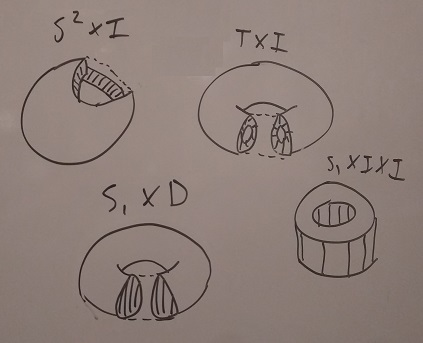
\includegraphics{IMG316}
  \newline
  \newpage
  \noindent
  \textbf{EXERCISE 3.17} If L is a line in the plane, describe the subspace topology it inherits from \(\mathbb{R}_l \times \mathbb{R}\) and from \(\mathbb{R}_l \times \mathbb{R}_l\), where \(\mathbb{R}_l\) is the real line in the lower limit topology. Note that the result depends on the slope of the line. In all cases, it is a familiar topology.
  \newline \newline
  If L is a vertical line, it inherits the standard topology on \(\mathbb{R}\) from \(\mathbb{R}_l \times \mathbb{R}\). Otherwise, it inherits  \(\mathbb{R}_l\). Unions of open intervals as well as interals closed at the lower limit are open sets in these non-vertical lines, all of which are open in the lower limit topology.
  \newline \newline
  L inherits \(\mathbb{R}_l\) from \(\mathbb{R}_l \times \mathbb{R}_l\) in all cases.
  \newpage
  \noindent
  \textbf{EXERCISE 3.18}
  Show that if X and Y are Hausdorff spaces, then so is the product space \(X \times Y\).
  \newline \newline
  Let X and Y be Hausdorff spaces.
  \newline
  Consider two distinct points \((x_1,y_1)\) and \((x_2,y_2)\) in the product space \(X \times Y\).
  \newline
  Since the points are distinct, either \(x_1 \neq x_2\) or \(y_1 \neq y_2\). \newline
  Without loss of generality, let \(x_1 \neq x_2\).
  \newline \newline
  Since X is Hausdorff \(\exists U, V \in X \ni x \in U\) and \(y \in V\).
  \newline
  Let \(U' = U \times Y\) and \(V' = V \times Y\).
  \newline
  \((x_1, y_1) \in U'\) and \((x_2,y_2) \in V'\)
  \newline
  Since U and V are disjoint, U' and V' are disjoint.
  \newline
  Thus, for any two distinct points in the product space \(X \times Y\), there exist disjoint subsets that contain those points.
  \newline \newline
  Therefore, the product space \(X \times Y\) is Hausdorff.
  \newpage
  \noindent
  \textbf{EXERCISE 3.19}
  Show that if A is closed in X and B is closed in Y, then \(A \times B\) is closed in \(X \times Y\).
  \newline \newline
  For sake of readability, let ' denote the complement of a set.
  \newline \newline
  Assume A and B are closed in X and Y respectively. \newline
  A' and B' are both open in X and Y.
  \newline
  So \(A' \times Y\) and \(X' \times B\) are open in \(X \times Y\).
  \newline
  This means \((A' \times Y)'\) and \((X' \times B)'\) are both closed in \(X \times Y\).
  \newline
  Thus, \((A' \times Y)' \cap (X' \times B)'\) is closed in \(X \times Y\).
  \[A \times B = A \times Y \cap X \times B\]
  \[A \times B = (A' \times Y)' \cap (X' \times B)'\]
  \(\therefore A \times B\) is closed in \(X \times Y\)
  \newline \(\blacksquare\)
  \newpage
  \noindent
  \textbf{EXERCISE 3.20}
  Show that if \(A \subseteq X\) and \(B \subseteq Y\), then Cl\((A \times B)\) = Cl\((A) \times\) Cl\((B)\).
  \newline \newline
  In Exercise 3.19, we have shown that if A is closed in X and B is closed in Y, then \(A \times B\) is closed in \(X \times Y\). \newline \newline
  Since \(A \subseteq\) Cl\((A)\) and \(B \subseteq\) Cl\((B)\)
  \(A \times B \subseteq\) Cl\((A) \times\) Cl\((B)\).
  \newline
  Cl\((A)\) and Cl\((B)\) are both closed, so Cl\((A) \times\) Cl\((B)\) is closed in \(X \times Y\).
  \newline
  Thus, Cl\((A \times B) \subseteq\) Cl\((A) \times\) Cl\((B)\).
  \newline \(\square\) \newline
  Let \((x,y) \in\) Cl\((A) \times\) Cl\((B)\).
  \newline
  Let H be an open set in \(X \times Y\) containing \((x,y)\).
  \newline
  Since H is open, it can be written as \(U \times V\), where U and V are open in X and Y respectively.
  \newline
  Since \(x \in Cl(A)\), U has to intersect A at a point other than x, by Theorem 2.8. Call it x'. (Axiom of choice)
  \newline
  \newline
  Thus, H intersects \(A \times B\) at \((x',y)\).
  \newline
  So for every open set H containing \((x,y)\), H intersects \(A \times B\) at a point other than \((x,y)\).
  \newline
  That makes \((x,y)\) a limit point of \(A \times B\).
  \newline
  So, by Theorem 2.8, \((x,y) \in\) Cl\((A \times B)\).
  \newline
  Thus, Cl\((A) \times\) Cl\((B) \subseteq\) Cl\((A \times B)\).
  \newline \(\square\) \newline
  \(\therefore\) Cl\((A \times B) =\) Cl\((A) \times\) Cl\((B)\).
  \newline \(\blacksquare\)
\end{document}
